\chapter{Plots}\label{ch:plots}

\section{nwlsmplot}

\texttt{nwlsmplot} draws the positions of the actors after \texttt{nwlsm} in the plane of two latent dimensions, with the ties as light lines (an undirected tie once, a directed tie as an arrow from the sender to the receiver, or with \opt{noarrows} as a line). \opt{dims(\# \#)} chooses the two dimensions (default 1 2), and \opt{mean} plots the mean of the aligned draws instead of the MKL positions. The positions are identified only up to rotation and reflection, so the orientation of the axes carries no meaning. Because only distances carry meaning, the two axes have the same scale by default (one unit is equally long on both), so that distances and the variance circles are drawn undistorted; \opt{noequal} switches this off.
\begin{figure}[ht]\centering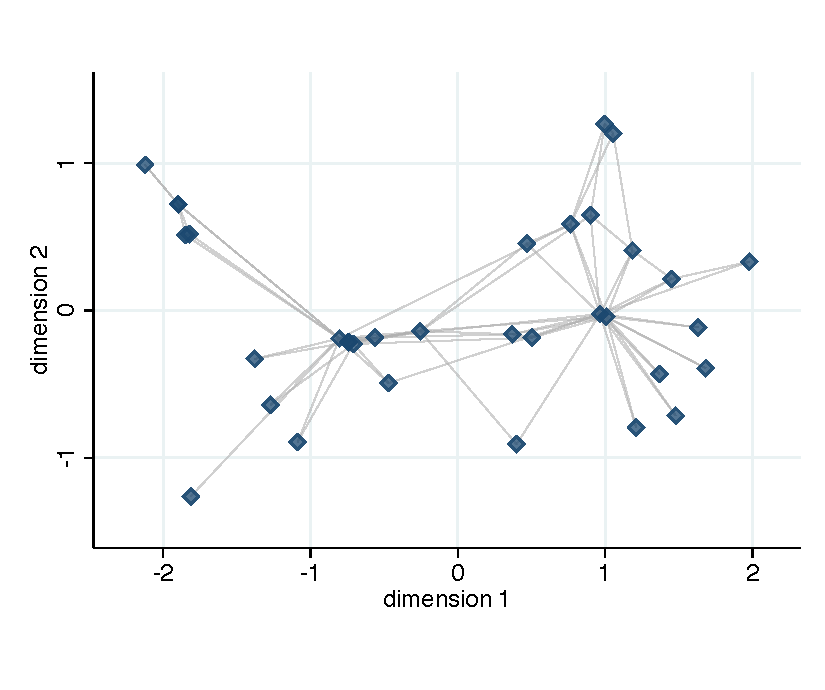
\includegraphics[width=0.8\textwidth]{fig/fig_karate_map.pdf}
\caption{\texttt{nwlsmplot} after the first model of the karate club: the 34 members in the latent space, the ties as lines.}\end{figure}

\paragraph{Colour, size and labels.} \opt{color(varname)} colours the actors by the values of a numeric or string variable (at most 15 values; the groups of a string variable are in alphabetical order); the legend shows the value labels of the variable, if it has them, and its variable label as the legend title. \opt{colors(list)} sets the colours of the groups of \opt{color()} or \opt{clusters}: a list of Stata colour names, or \texttt{gray}, where the groups differ by gray value and by marker (filled and hollow circles, diamonds, triangles, squares) so that they stay apart in a black-and-white print. \opt{clusters} colours the actors by their latent cluster (after \opt{clusters()}). \opt{size(spec)} sizes the actors by \texttt{sender}, \texttt{receiver} or \texttt{sociality} (posterior mean effects), by \texttt{influence} (the influence each actor exerts, after the influence model) or by a numeric variable. \opt{label(varname)} labels the actors with a string variable or a numeric variable (its value labels, or the numbers where it has none); \opt{labsize()} sets the size and \opt{labposition()} the clock position (0 to 12) of the labels, by default \texttt{auto}: each label goes to the clock position around its marker with the fewest other markers and already placed labels under it (up to 150 actors; larger networks use position 1).
\begin{figure}[ht]\centering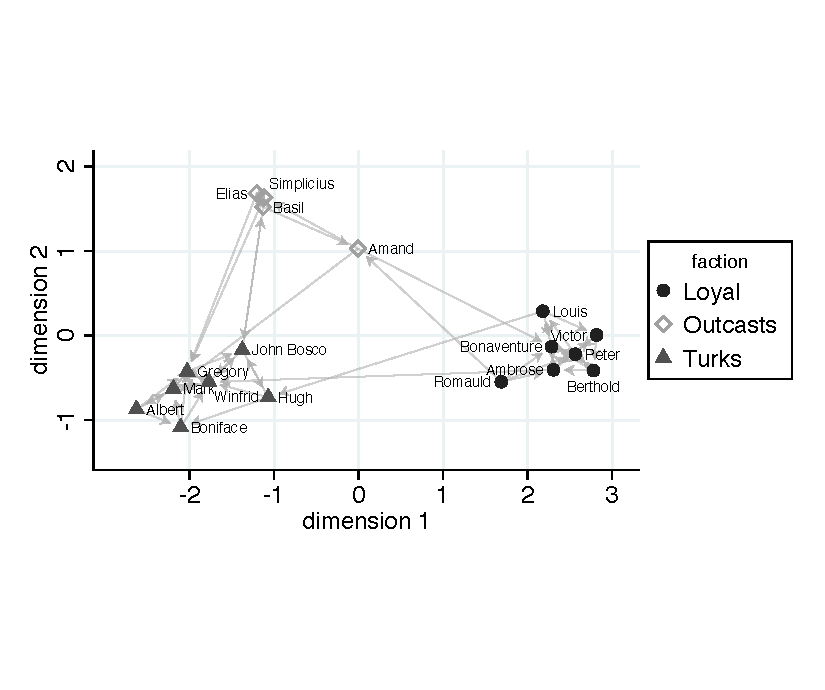
\includegraphics[width=0.85\textwidth]{fig/fig_monks_faction.pdf}
\caption{\texttt{nwlsmplot, color(faction) colors(gray) label(\_nwnode)}: the monks coloured by the observed faction, in gray for print. The groups are the same as the three clusters of Figure~\ref{fig:clusters}.}\end{figure}
\begin{figure}[ht]\centering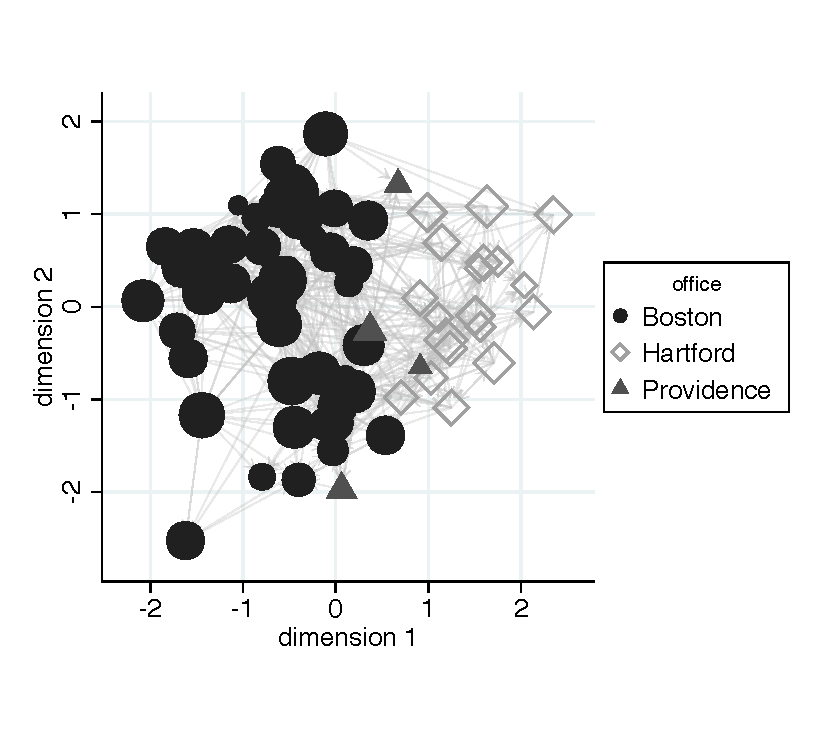
\includegraphics[width=0.85\textwidth]{fig/fig_lazega_map.pdf}
\caption{\texttt{nwlsmplot, color(office) colors(gray) size(sender)} after the fit with sender and receiver effects of the Lazega friendship network: the lawyers coloured by office, sized by the posterior mean sender effect.}\end{figure}

\paragraph{Ties.} \opt{noedges} draws no ties. \opt{arrows} and \opt{noarrows} control the arrow heads of directed networks (the default for directed networks is arrows), \opt{arrowsize()} their size; dense networks (more than 400 ties) get lighter tie lines and smaller arrow heads by default. \opt{edgecolor()} and \opt{edgewidth()} set the colour and the width of the lines.

\paragraph{Clusters and uncertainty.} After \opt{clusters()}, \opt{clustermeans} marks the posterior mean cluster means with a plus sign and \opt{circles} draws a circle around each with the square root of the posterior mean variance of the cluster as radius, as \texttt{plot.means} and \texttt{plot.vars} of \latentnet{}'s \texttt{plot.ergmm()} do; \opt{certainty} gives the markers an opacity by the largest posterior membership probability (four steps), so that uncertain actors look pale (Figure~\ref{fig:circles}). \opt{draws(\#)} (1 to 1000) draws a faint cloud of \# evenly spaced posterior draws of the positions under the actors, centred and rotated or reflected to the MKL positions. It needs the draws of the last fit in memory; if they are gone, or belong to another fit than the one in \texttt{e()}, \texttt{nwlsmplot} stops with an error.
\begin{figure}[ht]\centering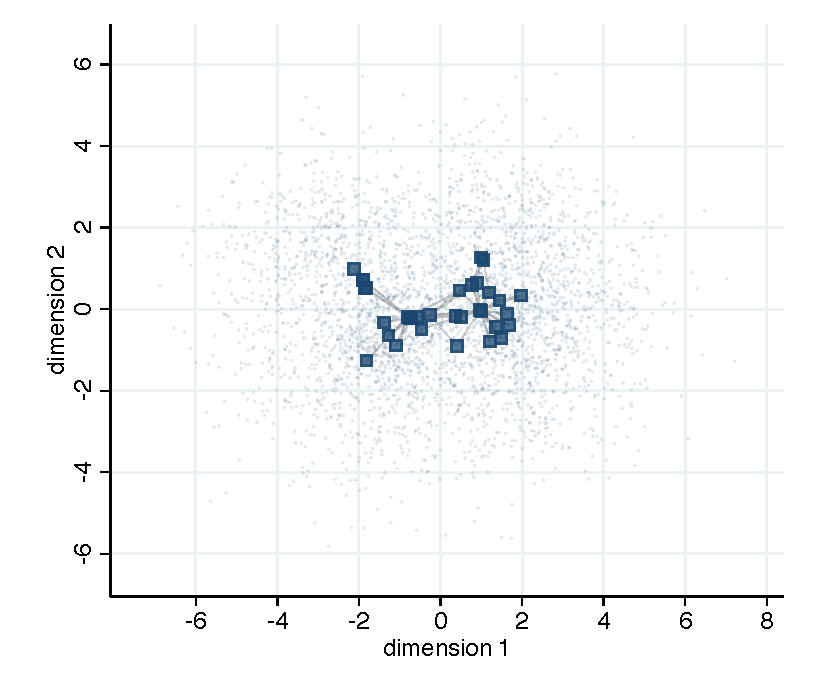
\includegraphics[width=0.85\textwidth]{fig/fig_karate_draws.pdf}
\caption{\texttt{nwlsmplot, draws(100)} on the karate club: 100 posterior draws of the positions behind the estimated positions. The estimated positions sit in the middle of a much wider cloud: the map is a tidy summary, but the data do not pin down the position of an individual actor.}\end{figure}

Compared with \texttt{plot.ergmm()} of \latentnet{}, not offered are pie charts of the membership probabilities (see \opt{certainty}), density plots, plots of one latent dimension, 3-D plots, \texttt{Z.ref} and \texttt{zoom.on}.

\section{The plots of the estat commands and nwlsmselect}

\texttt{estat mcmcdiag, graph} draws the trace plots, \texttt{estat gof, plot} the box plots of the goodness of fit, \texttt{estat ppcheck, graph} the calibration plot, \texttt{estat influence, graph} observed against predicted outcomes, and \texttt{nwlsmselect, graph} the BIC against the number of clusters. They appear in the chapters where the commands are described.

\section{Name, saving and export}\label{sec:plotconv}

\texttt{nwlsmplot} follows the convention of the plot commands of the family. \opt{name(name)} names the graph in memory; \opt{saving(filename)} (a \texttt{twoway} option) saves it as a \texttt{.gph} file, and \opt{export(filename)} exports it with \texttt{graph export}, the extension of the file name (\texttt{.pdf}, \texttt{.png}, \dots) setting the format; options of \texttt{graph export} may follow after a comma, as in \opt{export(positions.png, width(1200))}. The graphs of the \texttt{estat} commands take \opt{name()}, and \texttt{nwlsmselect} takes \opt{gname()} and \opt{gopts()}; such a graph is exported with \texttt{graph export} and, to change its size, \texttt{graph display} with \texttt{xsize()} and \texttt{ysize()} first. Other options of \texttt{twoway}, such as \texttt{title()}, \texttt{scheme()} or \texttt{xsize()}, come last in \texttt{nwlsmplot} and override the defaults; titles, subtitles, axis titles and legend titles are black by default in all of these plots, also a \texttt{title()} or \texttt{subtitle()} you give to \texttt{nwlsmplot} (unless it has its own \texttt{color()}). The figures of this manual were made with the scheme \texttt{s1network} of the core package and exported to PDF:
\begin{lstlisting}
. nwlsmplot, color(faction) colors(gray) label(_nwnode) title("") xsize(5.5) ysize(4.6) export(fig_monks_faction.pdf)
. estat ppcheck, graph name(m_ppcheck)
. graph display m_ppcheck, xsize(5) ysize(4)
. graph export fig_monks_ppcheck.pdf, name(m_ppcheck) replace
\end{lstlisting}
